\newpage
\section{Administration système}
Le pôle administration système joue un rôle essentiel dans le maintien en condition opérationnelle des systèmes informatiques de l'entreprise.
Il est responsable de la gestion des sauvegardes et de la récupération des données, assurant ainsi la disponibilité et l'intégrité des informations cruciales.
De plus, il effectue également l'inventaire des équipements et des logiciels, ce qui permet de maintenir une visibilité précise sur les ressources technologiques de l'entreprise.
Grâce à ces responsabilités, le pôle administration système contribue à assurer la continuité des activités, la sécurité des données et la performance des systèmes, ce qui est essentiel pour la productivité et la réussite globale de l'organisation.

Le pôle d'administrateurs système est composé d'une seule personne, Delgutte Théo.
J'ai eu l'occasion de l'assister dans sa mission continue de maintien en condition opérationnelle de la partie informatique de l'entreprise.

\subsection{Objectifs initiaux}
\subsubsection{Réduction des risques}
L'objectif de mon stage était d'atténuer les divers risques potentiels liés à la cyberattaque et à la perte de données.

Ci-dessous une liste des risques identifiés en amont de mon stage :
\begin{itemize}
    \item \textbf{Vulnérabilités Systèmes}
    \item \textbf{Attaques par Hameçonnage}
    \item \textbf{Perte de Données}
    \item \textbf{Accès Non Autorisés}
    \item \textbf{Malwares et Logiciels Malveillants}
    \item \textbf{Défaillance Matérielle}
    \item \textbf{Fuites d'Informations}
\end{itemize}

\subsubsection{Attraction des clients}
De plus, certains clients travaillant avec des données sensibles et des secrets industriels ont manifesté leur intérêt pour l'utilisation du logiciel DiagFit.
Toutefois, ils ont émis une condition spécifique : \hyperref[iso]{l'obtention de la certification ISO 27001 [1]}.
Cette exigence aurait pu constituer un élément différenciateur et potentiellement plus vendeur pour le logiciel, renforçant ainsi son attrait auprès de clients soucieux de la sécurité de leurs données.

\newpage

\subsection{Missions effectuées}
Dans le cadre de mon stage, j'ai entrepris diverses missions visant à améliorer la fonctionnalité, la stabilité et la gestion globale de notre environnement informatique d'Amiral Technologies.

\subsubsection{Gestion de l'infrastructure et de l'inventaire}
J'ai contribué à l'amélioration de notre infrastructure informatique en mettant en place des actions ciblées pour optimiser son fonctionnement.
Cela incluait notamment la résolution d'un problème lié à notre serveur web qui restreignait les modifications par les collaborateurs.
Pour résoudre ce problème, j'ai configuré un serveur de développement dédié, permettant de tester les changements avant leur application sur le site en production.
J'ai également migré les URL en adaptant la base de données du site via des requêtes SQL.

En parallèle, j'ai supervisé l'inventaire matériel et utilisateurs pour une meilleure gestion des ressources et des droits d'accès.
J'ai veillé à ce que les droits d'accès des utilisateurs soient en conformité avec les politiques de sécurité et proposé la conception d'une base de données d'inventaire pour centraliser et suivre les attributions aux utilisateurs.

Enfin, j'ai travaillé sur l'optimisation du schéma réseau en identifiant et en documentant minutieusement les adresses IP associées à chaque machine et service de l'entreprise.
Le schéma de l'infrastructure de l'entreprise est disponible \hyperref[infra]{en annexe}.

Le fonctionnement des services se faisait sous une structure appelée cluster.
La charge de travail était donnée à deux serveurs "maîtres" qui à leur tour répartissaient les tâches à leurs serveurs "esclaves".
Cette structure est souvent utilisée pour permettre de diviser la charge de travail entre plusieurs serveurs et de ne pas dépendre que d'un seul élément pour le fonctionnement des services.
Un schéma de la structure est disponible \hyperref[balancer]{en annexe également}.

\subsubsection{Approche de la Cybersécurité au Quotidien}
La sécurité informatique étant une priorité chez Amiral Technologies, j'ai contribué à mettre en place une approche pratique pour garantir la protection des systèmes et des données des divers clients.
Pour cela, nous avons initié plusieurs axes d'action.

En premier lieu, j'ai participé à la collecte et à la synthèse de documents clés en lien avec \hyperref[iso]{la norme ISO27001}, ce qui nous a permis d'acquérir une solide compréhension des meilleures pratiques en matière de sécurité.

J'ai également eu l'opportunité de participer à une conférence de la Direction du Renseignement et de la Sécurité de la Défense (DRSD), qui m'a apporté des perspectives concrètes sur les enjeux de cybersécurité et d'espionnage industriel international.

Un aspect clé de notre approche a été l'intégration de l'outil Sophos Zero Trust Network Access (ZTNA), qui répond à nos besoins croissants de protection des données et systèmes.
J'ai ensuite organisé une présentation approfondie de l'outil Sophos ZTNA pour assurer sa compréhension et son utilisation par tous les collaborateurs.

Parallèlement, nous avons renforcé notre surveillance en mettant en place Wazuh.
Cette solution nous a permis d'améliorer la détection des menaces en centralisant la surveillance via un serveur Wazuh Manager et un Wazuh Indexer.
L'installation automatisée des agents Wazuh sur les ordinateurs a assuré une surveillance constante et réactive.

Enfin, pour faciliter la gestion et le partage de connaissances, nous avons créé une documentation interne à l'aide de Docusaurus.
Cette plateforme, hébergée sur un PC réhabilité sous Ubuntu, a été organisée en deux parties : une pour les employés et une pour les administrateurs système, couvrant divers scénarios et procédures liées à notre environnement informatique.

Cette approche holistique de la cybersécurité a permis de renforcer notre positionnement tout en garantissant la stabilité et la performance de notre environnement informatique.

\subsection{Retour et critiques sur le projet}
Après environ un mois et demi de mise en place du projet, nous avons organisé une réunion rétrospective pour évaluer son utilité et son impact.
Il est apparu que malgré nos efforts, le projet a entraîné certaines difficultés pour de nombreux collègues lors de sa mise en œuvre.

\subsubsection{Effets contradictoires sur la sécurité}
Les mesures mises en place n'ont pas toujours contribué de manière significative à la réduction des risques, et dans certains cas, elles ont même posé de nouvelles contraintes aux collaborateurs.
Par exemple, l'utilisation d'outils complexes a parfois créé une dépendance envers une seule personne, en l'occurrence l'administrateur système Théo Delgutte.
Cette situation est devenue problématique lors de ses périodes de congés, entraînant des retards et des perturbations dans les opérations.

\subsubsection{Perte de stabilité}
Un autre défi que nous avons rencontré concerne la stabilité des outils utilisés par les collaborateurs de l'entreprise.
Les modifications apportées en cours de route par le sysadmin ont souvent impacté les ressources et les services, générant ainsi une instabilité préjudiciable au bon fonctionnement quotidien.
Cette instabilité a été particulièrement préoccupante pour les employés travaillant à distance, car elle a rendu difficile voire impossible le travail en télétravail sans préavis.

\subsubsection{Perte de l'autonomie}
La décision de limiter les accès aux ressources a également eu des répercussions négatives sur le fonctionnement général de l'entreprise.
Étant donné que le développement de différentes parties du projet est interconnecté et que la documentation d'une partie peut être utile à un autre groupe de personnes, la limitation des accès a entravé la fluidité de la collaboration.
De plus, en tant qu'entreprise de petite taille, les contraintes imposées par cette limitation d'accès semblaient disproportionnées par rapport à d'autres risques potentiellement plus importants.

\newpage

\subsection{Modification des objectifs}
Cette section aborde les ajustements apportés aux objectifs initiaux, visant à résoudre les problèmes identifiés et à reprendre les points bloquants du projet en main.

\subsubsection{Éducation à la cybersécurité}
Au cœur de la cybersécurité réside une composante essentielle : l'éducation des employés pour réduire les risques potentiels.
Dans cette optique, j'ai joué un rôle clé en sensibilisant l'entreprise à l'importance de la cybersécurité grâce à des présentations hebdomadaires.
Ces sessions ont couvert une variété de sujets visant à renforcer la vigilance et les bonnes pratiques parmi les collaborateurs.

Parmi les thèmes abordés, j'ai présenté un guide appréhensible sur l'hygiène de la cybersécurité.
Cela comprenait des conseils pratiques pour naviguer en toute sécurité en ligne, en mettant l'accent sur la prudence face au public, la reconnaissance des extensions de fichiers, la détection d'URL malveillantes et l'utilisation de bloqueurs de traqueurs pour contrôler les publicités et les cookies.

Une attention particulière a été portée sur l'utilisation de gestionnaires de mots de passe pour renforcer la sécurité des comptes en ligne.
Nous avons également abordé les risques liés aux emails malveillants, aux spams et au phishing, en fournissant des méthodes pour les identifier et les éviter.

Un volet de mon travail a consisté à explorer et utiliser l'outil Gophish pour la création d'une campagne de sensibilisation interne sur le phishing.
J'ai récupéré le code source de sites officiels de Microsoft et Gitlab ainsi que d'emails officiels des mêmes groupes dans le but de montrer comment des attaquants pourraient collecter des informations sensibles.
Par la suite, j'ai conçu un message contenant un lien malicieux pour simuler une campagne de phishing.
On peut voir ci-dessous le sondage que j'ai envoyé aux membres de l'entreprise concernant le lien présent dans mon message qui ne concernaît que les membres de l'entreprise présents dans les locaux au moment de la campagne.

\begin{figure}[ht!]
    \centering
    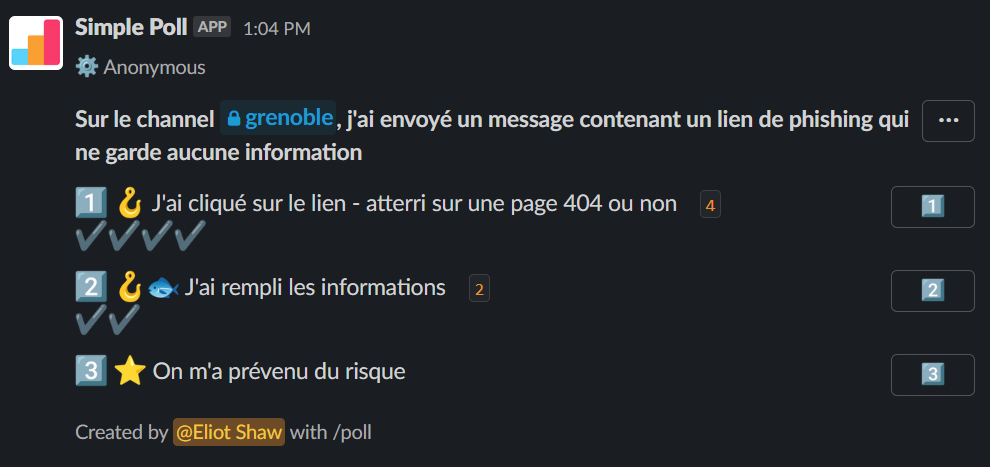
\includegraphics[width=0.66\textwidth]{paper/figures/poll.png}
    \caption{Résultats du sondage concernant le lien de phishing}
    \label{fig:poll}
\end{figure}

Une présentation détaillée a ensuite été faite, montrant les résultats ayant pour objectif de convaincre les employés qu'une attaque informatique peut arriver à tout moment et commettre une imprudence dans le cadre du travail est possible.
Le but de la présentation n'est pas de stigmatiser les personnes s'ayant fait avoir par la campagne mais de permettre aux employés d'aborder le sujet sans tabou pour les habituer à annoncer s'ils ont été victimes d'une attaque.


\subsubsection{Mise en place d'une infrastructure alternative}
Les outils trop complexes à maintenir en condition opérationnelle pour leur coût humain ont été retirés : les agents Wazuh et Sophos ZTNA ont donc été désinstallés pour cette raison.

Un membre de l'entreprise, Rémy Dufrenoy, a également pris de son temps de travail pour créer une nouvelle infrastructure, plus simple pour pouvoir bénéficier d'environnements de travail stables sur lequels ses collègues et lui pourront travailler.

\subsubsection{Modification des droits et autorisations}
Les employés d'Amiral Technologies ont également bénéficié de plus de droits d'accès aux ressources générées par leurs collègues permettant une efficacité de travail plus grande.

En parallèle, un groupe de responsables de l'administration du système fut mis en place pour limiter la création d'un point unique de dépendances.
Une base de données sécurisée de mots de passe contenant les identifiants administrateur pour les ressources fut également créée et partagée entre les responsables.

\subsection{Enseignements appris}
Dans la section qui suit, je partagerai les enseignements que j'ai acquis au cours de cette expérience.

\subsubsection{Shéma des prises de décisions}
Dans ce projet j'ai eu l'occasion d'observer le processus de prises de décisions évolutives.
Le shéma prend en compte le retour d'experience des utilisateurs de l'entreprise pour définir de nouveaux objectifs et diagnostics des besoins.

\begin{figure}[ht!]
    \centering
    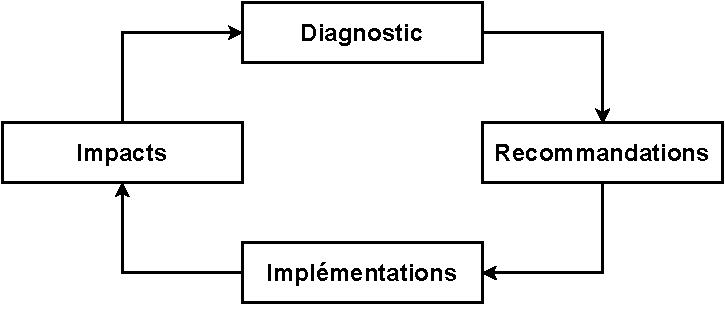
\includegraphics[width=0.5\textwidth]{paper/figures/boucle.pdf}
    \caption{Processus de prise de décisions}
    \label{fig:boucle}
\end{figure}

On peut illuster la première étape du processus décisionnel qui résulte de la craînte de ne pas conquérir de nouvelles parts de marché si les normes de sécurité informatique n'étaient pas obtenues.
\newpage
\begin{figure}[ht!]
    \centering
    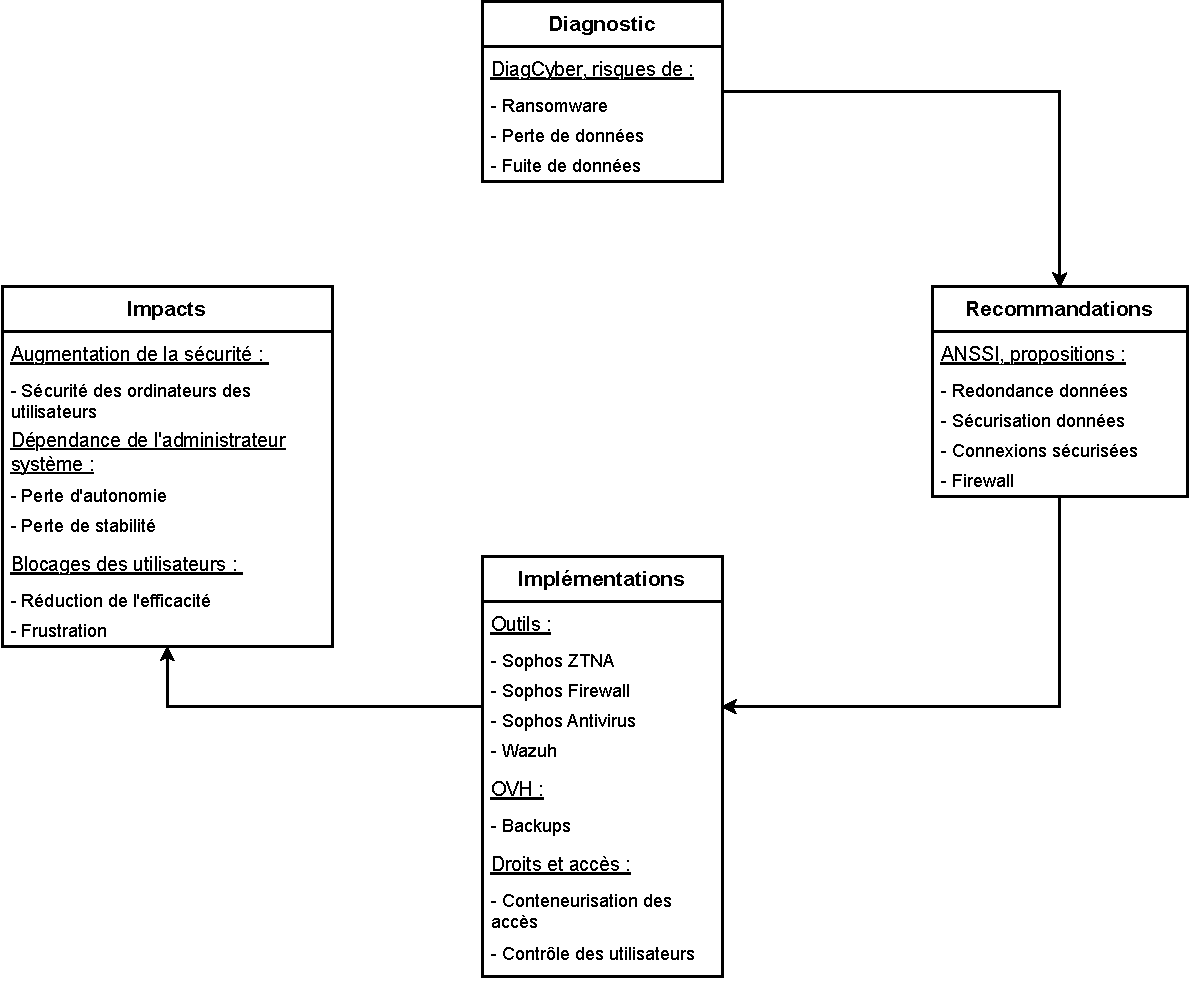
\includegraphics[width=0.8\textwidth]{paper/figures/boucle1.pdf}
    \caption{Première boucle du processus décisionnel}
    \label{fig:boucle1}
\end{figure}

Suite aux retours des employés, nous avons découvert plusieurs points importants non étudiés lors de la pemière observation qui a engendré en une modification des priorités.

\begin{figure}[ht!]
    \centering
    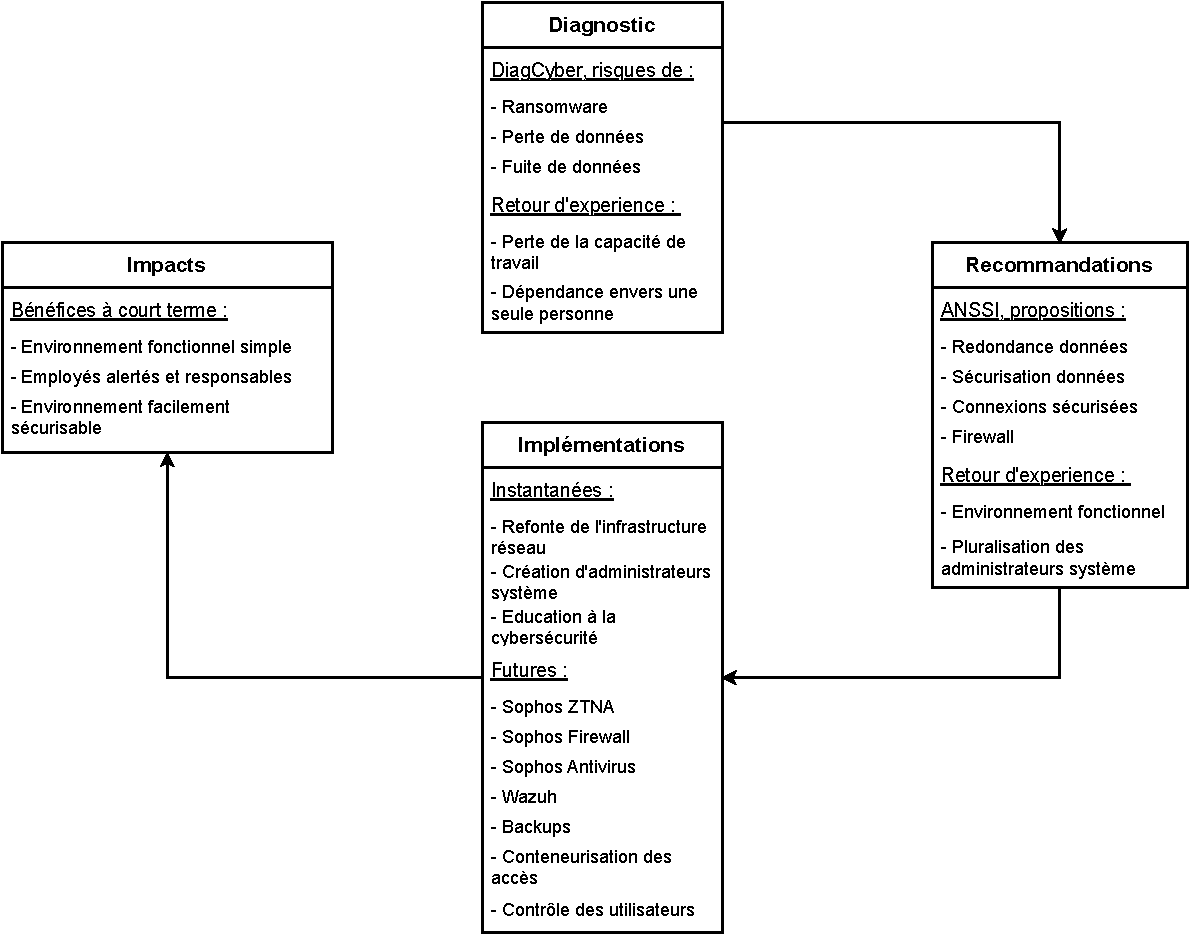
\includegraphics[width=0.8\textwidth]{paper/figures/boucle2.pdf}
    \caption{Seconde boucle du processus décisionnel}
    \label{fig:boucle2}
\end{figure}

\subsubsection{Communication Essentielle}
Lorsque des problèmes ont conduit à des retours en arrière, l'absence de communication adéquate a souvent été à l'origine de ces situations problématiques.
lors de la mise en place de nouvelles restrictions d'accès, les utilisateurs n'ont pas été prévenus des changements à venir.
Cela a provoqué des frustrations et des interruptions dans leur travail quotidien.

Convaincre plutôt qu'imposer est essentiel pour éviter de mécontenter les utilisateurs des services concernés : au lieu d'imposer des nouvelles politiques de sécurité, il serait préférable de présenter les raisons derrière ces changements.

L'importance de l'aspect humain, même dans le domaine de l'administration système, est devenue évidente.
Par exemple, lorsque le système d'exploitation d'un ordinateur ne fonctionnait plus en raison d'un problème matériel, expliquer aux utilisateurs la nature du problème.

Maintenir une communication transparente avec les utilisateurs et expliquer les problèmes rencontrés contribue à renforcer leur confiance et leur satisfaction.

\subsubsection{L'isopérimétrie dans le monde de l'entreprise}
Dans le contexte professionnel actuel, équilibrer l'efficacité au travail et la cybersécurité est crucial.
Les entreprises font face à des menaces de cybersécurité de plus en plus sophistiquées, nécessitant une protection robuste.
Les attaques informatiques évoluent constamment, rendant difficiles la prévention de chaque menace potentielle.

Les administrateurs système jouent un rôle central dans cet équilibre.
Responsables de la sécurité et de la performance des systèmes, ils doivent concevoir des environnements sûrs tout en facilitant la productivité.
Le défi réside dans la recherche du bon équilibre entre des mesures de sécurité strictes et des opérations fluides.

Cela exige des solutions astucieuses de la part des administrateurs système.
L'objectif ultime étant de créer un environnement où la sécurité est maximisée, tout préservant la capacité à livrer de la valeur.





